\documentclass[aspectratio=169]{beamer}
\usetheme{Madrid}
\usecolortheme{default}
\usepackage{tikz}
\usetikzlibrary{shapes.geometric, arrows.meta, positioning, fit, backgrounds, calc, shapes.symbols}
\usepackage{listings}
\usepackage{booktabs}

\title{Vector-ARC RAG System Architecture}
\subtitle{Adaptive Replacement Semantic Caching}
\author{System Architecture Review}
\date{\today}

\begin{document}

\begin{frame}
    \titlepage
\end{frame}

\begin{frame}{Motivation \& System Goals}
    \begin{itemize}
        \item \textbf{Problem 1:} Standard RAG systems suffer from high latency and LLM API costs for repeated or semantically similar queries.
        \item \textbf{Problem 2:} Existing semantic caches (e.g., SCRL) suffer from unbounded memory growth due to storing large embedding vectors for evicted items in their tracking history.
        \item \textbf{Solution (Vector-ARC):} An $O(1)$-memory semantic cache that adapts to recency and frequency, integrated with a hybrid cold storage RAG pipeline.
        \item \textbf{Key Design Choices (As Implemented):}
        \begin{itemize}
            \item Q-to-Q (Query-to-Query) comparison for semantic cache hits.
            \item Full LLM Answer Caching to bypass LLM generation entirely ($\sim$300x speedup).
            \item SimHash-based ghost caches to enable semantic adaptation with bounded $O(1)$ memory overhead.
        \end{itemize}
    \end{itemize}
\end{frame}

\begin{frame}{Core Technologies, Frameworks \& Justifications}
    \begin{itemize}
        \item \textbf{Language \& Orchestration:} Python (modular design via \texttt{rag\_coordinator.py})
        \item \textbf{Embeddings:} \texttt{SentenceTransformers} (\texttt{all-MiniLM-L6-v2})
        \begin{itemize}
            \item \textit{Why:} 384-D dense vectors provide high semantic density and fast CPU/GPU inference.
        \end{itemize}
        \item \textbf{Cold Storage (Hybrid \texttt{HybridColdStorage}):} 
        \begin{itemize}
            \item \textbf{Dense:} \texttt{FAISS} (\texttt{IndexFlatIP}). \textit{Why:} Exact inner-product search is optimal for small corpora (e.g., IIT Dharwad rules) without the memory/build overhead of HNSW.
            \item \textbf{Sparse:} \texttt{rank\_bm25}. \textit{Why:} Okapi BM25 guarantees exact keyword and acronym matching.
        \end{itemize}
        \item \textbf{LLM Engine:} Google GenAI API. \textit{Why:} High-quality text synthesis for answer generation.
        \item \textbf{Persistence:} NumPy (\texttt{.npy}) \& JSON. \textit{Why:} JSON for metadata readability, \texttt{.npy} for exact, compact float32 vector storage.
    \end{itemize}
\end{frame}

\begin{frame}{Overall System Architecture}
    \begin{center}
    \resizebox{0.95\textwidth}{!}{
    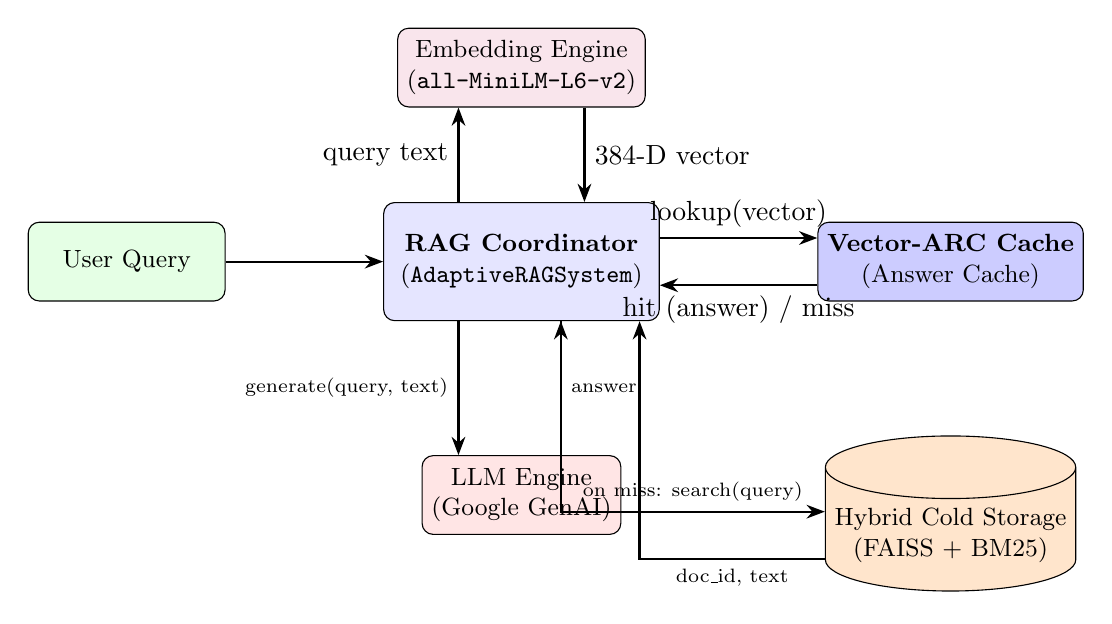
\begin{tikzpicture}[
        node distance=1.2cm and 2cm,
        box/.style={draw, rounded corners, fill=blue!10, minimum width=2.5cm, minimum height=1cm, align=center, font=\small},
        db/.style={cylinder, draw, shape border rotate=90, aspect=0.25, fill=orange!20, minimum height=1.5cm, minimum width=2.5cm, align=center, font=\small},
        arrow/.style={-Stealth, thick}
    ]
        
        \node[box, fill=green!10] (user) {User Query};
        \node[box, right=of user, minimum width=3.5cm, minimum height=1.5cm] (coord) {\textbf{RAG Coordinator}\\(\texttt{AdaptiveRAGSystem})};
        \node[box, above=of coord, fill=purple!10] (embed) {Embedding Engine\\(\texttt{all-MiniLM-L6-v2})};
        \node[box, right=of coord, fill=blue!20] (cache) {\textbf{Vector-ARC Cache}\\(Answer Cache)};
        \node[db, below=of cache, yshift=-0.5cm] (hybrid) {Hybrid Cold Storage\\(FAISS + BM25)};
        \node[box, below=of coord, fill=red!10, yshift=-0.5cm] (llm) {LLM Engine\\(Google GenAI)};
        
        \draw[arrow] (user) -- (coord);
        
        \draw[arrow] ([xshift=-0.8cm]coord.north) -- ([xshift=-0.8cm]embed.south) node[midway, left] {query text};
        \draw[arrow] ([xshift=0.8cm]embed.south) -- ([xshift=0.8cm]coord.north) node[midway, right] {384-D vector};
        
        \draw[arrow] ([yshift=0.3cm]coord.east) -- ([yshift=0.3cm]cache.west) node[midway, above] {lookup(vector)};
        \draw[arrow] ([yshift=-0.3cm]cache.west) -- ([yshift=-0.3cm]coord.east) node[midway, below] {hit (answer) / miss};
        
        \draw[arrow] ([xshift=0.5cm]coord.south) |- ([yshift=0.3cm]hybrid.west) node[pos=0.75, above, font=\scriptsize] {on miss: search(query)};
        \draw[arrow] ([yshift=-0.3cm]hybrid.west) -| ([xshift=1.5cm]coord.south) node[pos=0.25, below, font=\scriptsize] {doc\_id, text};
        
        \draw[arrow] ([xshift=-0.8cm]coord.south) -- ([xshift=-0.8cm]llm.north) node[midway, left, font=\scriptsize] {generate(query, text)};
        \draw[arrow] ([xshift=0.5cm]llm.north) -- ([xshift=0.5cm]coord.south) node[midway, right, font=\scriptsize] {answer};
        
    \end{tikzpicture}
    }
    \end{center}
\end{frame}

\begin{frame}{Request Routing \& Execution Pipeline}
    \begin{center}
    \resizebox{0.9\textwidth}{!}{
    \begin{tikzpicture}[
        node distance=0.6cm and 0.8cm,
        step/.style={draw, rectangle, fill=gray!10, align=center, rounded corners, minimum height=0.8cm, font=\small},
        decision/.style={draw, diamond, fill=yellow!20, aspect=2.5, align=center, font=\scriptsize},
        arrow/.style={-Stealth, thick}
    ]
        \node[step] (q) {1. Receive Query};
        \node[step, right=of q] (e) {2. Embed Query (384-D)};
        \node[step, right=of e] (scan) {3. ENN Cache Scan};
        \node[decision, below=of scan] (check) {Score $\geq 0.90$ \\ \& Margin $\geq 0.05$?};
        
        \node[step, fill=green!20, left=of check, xshift=-1cm] (hit) {4a. Cache Hit!\\Return cached \texttt{answer}};
        
        \node[step, fill=red!10, below=of check] (hybrid) {4b. Cache Miss!\\Hybrid DB Search};
        \node[step, fill=red!10, left=of hybrid, xshift=-0.5cm] (admit1) {5. Admit w/o LLM\\\texttt{admit\_to\_cache}};
        \node[step, fill=red!10, above=of admit1] (llm) {6. LLM Synthesis\\Generate \texttt{answer}};
        \node[step, fill=blue!10, above=of llm] (admit2) {7. Update Cache\\\texttt{update\_answer}};
        
        \draw[arrow] (q) -- (e);
        \draw[arrow] (e) -- (scan);
        \draw[arrow] (scan) -- (check);
        
        \draw[arrow] (check) -- node[above] {Yes} (hit);
        \draw[arrow] (check) -- node[right] {No} (hybrid);
        \draw[arrow] (hybrid) -- (admit1);
        \draw[arrow] (admit1) -- (llm);
        \draw[arrow] (llm) -- (admit2);
        \draw[arrow] (admit2) -- (hit);
        
    \end{tikzpicture}
    }
    \end{center}
\end{frame}

\begin{frame}{Embeddings \& Similarity Search}
    \begin{itemize}
        \item \textbf{Generation:} \texttt{EmbeddingEngine} converts text into 384-D dense vectors. Vectors are L2-normalized upon generation.
        \item \textbf{Cache Search (Q-to-Q Comparison):}
        \begin{itemize}
            \item The incoming query vector is compared against all cached \textit{query} vectors (not document vectors) using a fast NumPy dot product.
            \item This ensures high similarity scores ($> 0.90$) for paraphrased queries.
        \end{itemize}
        \item \textbf{Cold Storage Search:}
        \begin{itemize}
            \item FAISS performs \texttt{IndexFlatIP} (inner product) search between the query vector and all corpus document vectors for semantic retrieval.
        \end{itemize}
    \end{itemize}
\end{frame}

\begin{frame}{Semantic vs. Retrieval Caching: Why NO Top-k in Cache?}
    \begin{block}{The Question}
    Why doesn't the cache return the Top-k entries above a threshold and fill the rest from the cold database?
    \end{block}
    
    \begin{itemize}
        \item \textbf{Answer Caching vs Retrieval Caching:} We cache the \textit{full LLM-generated answer}, making this a Level 1 Answer Cache.
        \item \textbf{Retrieval Caching (Top-k):} Caches \textit{document chunks} to feed into an LLM context window. It still requires a $\sim$300ms LLM call.
        \item \textbf{Recall Optimality:} A cache hit implies we already searched the entire cold storage on a prior miss, found the optimal document, and synthesized an optimal answer. Returning multiple cached answers and re-running the LLM defeats the immense latency speedup.
    \end{itemize}
\end{frame}

\begin{frame}{Cache Hit/Miss Decision (Threshold \& Margin Guard)}
    \begin{itemize}
        \item \textbf{Exact Nearest Neighbor (ENN):} Cache search uses an exact NumPy matrix dot product. Approximate search (HNSW) is unnecessary and slower for small capacities ($<10,000$).
        \item \textbf{Strict Threshold ($0.90$):} Ensures high semantic equivalence.
        \item \textbf{Margin-Based Guardrail ($\epsilon = 0.05$):}
        \begin{itemize}
            \item Prevents false positives without the latency penalty of a Cross-Encoder.
            \item \textbf{Calculation:} Margin = (Top 1 Score) - (Top 2 Score).
            \item If Margin $< 0.05$, the match is flagged as \textit{ambiguous} (query sits between two distinct cached concepts).
            \item The system forcibly triggers a Cache Miss, prioritizing correctness over latency.
        \end{itemize}
    \end{itemize}
\end{frame}

\begin{frame}{Cache Metadata \& Data Flow}
    \begin{itemize}
        \item \textbf{Data Flow:} User Query $\rightarrow$ Embedding $\rightarrow$ Cache Search $\rightarrow$ (if miss) Cold Storage Search $\rightarrow$ LLM Synthesis $\rightarrow$ Cache Admission $\rightarrow$ Response.
        \item \textbf{Cache Payload (Hot Tier Metadata):}
        \begin{itemize}
            \item \texttt{text}: Raw context retrieved from the cold storage.
            \item \texttt{vector}: 384-dimensional query embedding.
            \item \texttt{answer}: The full LLM-synthesized response.
            \item \texttt{expires\_at}: Unix timestamp for TTL expiry.
        \end{itemize}
        \item \textbf{Cache Payload (Ghost Tier Metadata):}
        \begin{itemize}
            \item MD5 Hash string (key) $\rightarrow$ 64-bit uint64 SimHash (8 bytes).
        \end{itemize}
    \end{itemize}
\end{frame}

\begin{frame}{Cache Eviction \& ARC Policy}
    \begin{itemize}
        \item \textbf{Adaptive Replacement Cache (ARC):} Dynamically balances between recency and frequency based on workload patterns.
        \item \textbf{T1 (Recency):} Items seen exactly once.
        \item \textbf{T2 (Frequency):} Items seen at least twice.
        \item \textbf{Boundary Parameter ($p$):} Determines the target size of T1 ($0 \le p \le C$).
        \item \textbf{Eviction Workflow:}
        \begin{itemize}
            \item If $T1 + T2 = C$ and a new miss arrives, an item is evicted.
            \item If $|T1| > p$, the Least Recently Used (LRU) item from T1 is evicted to B1.
            \item Otherwise, the LRU item from T2 is evicted to B2.
        \end{itemize}
    \end{itemize}
\end{frame}

\begin{frame}{The Ghost Cache: Exact Match + SimHash}
    \begin{block}{The O(1) Memory Solution}
        Storing evicted 384-D vectors would cause unbounded $O(N)$ memory growth. Instead, we compress the evicted vector into a \textbf{SimHash} (64-bit uint64).
    \end{block}
    
    Ghost cache hits determine how $p$ adapts. They are evaluated in a two-tier priority system:
    \begin{enumerate}
        \item \textbf{Priority 1: Exact Match (O(1) Dictionary Lookup)}
        \begin{itemize}
            \item Dictionary key is the MD5 hash of the normalized query.
        \end{itemize}
        \item \textbf{Priority 2: Semantic Match (Hamming Distance)}
        \begin{itemize}
            \item Compares incoming query's SimHash against ghost SimHashes using fast bitwise operations (\texttt{bin(a\textasciicircum b).count('1')}).
            \item If Hamming Distance $\le 10$, we declare a Semantic Ghost Hit.
        \end{itemize}
    \end{enumerate}
    \textbf{Result:} ARC adapts even for \textit{paraphrases} of evicted queries!
\end{frame}

\begin{frame}{Hybrid Cold Storage Pipeline}
    \begin{itemize}
        \item \textbf{Motivation:} Dense vectors miss exact technical IDs/acronyms. Sparse vectors miss semantic intent and synonyms.
        \item \textbf{Implementation (\texttt{HybridColdStorage}):} Runs FAISS and BM25 in parallel and fuses results via \textbf{Reciprocal Rank Fusion (RRF)}.
        \item \textbf{RRF Formula:} $Score = \frac{1}{60 + Rank_{BM25}} + \frac{1}{60 + Rank_{FAISS}}$
        \item \textbf{Implementation Trade-offs:}
        \begin{itemize}
            \item \texttt{IndexFlatIP} is used for FAISS (exhaustive search).
            \item The FAISS index is built \textit{lazily} on the first miss to save initialization overhead for applications that might solely hit the cache early on.
        \end{itemize}
    \end{itemize}
\end{frame}

\begin{frame}{Cache Update \& Persistence Workflow}
    \begin{itemize}
        \item \textbf{Separated Admission (\texttt{admit\_to\_cache} vs \texttt{update\_answer}):}
        \begin{itemize}
            \item \texttt{retrieve()} admits the entry with \texttt{answer=None} immediately upon finding the document from cold storage.
            \item After LLM generation, \texttt{update\_answer()} mutates the hot cache entry in-place.
            \item This prevents redundant eviction/admission cycles for the same query.
        \end{itemize}
        \item \textbf{Time-To-Live (TTL):}
        \begin{itemize}
            \item Evaluated lazily during \texttt{VectorARC.get()}.
            \item Expired items are dropped entirely (not pushed to ghost lists), as TTL expiry is a data-freshness event, not a capacity-contention event.
        \end{itemize}
        \item \textbf{State Persistence:}
        \begin{itemize}
            \item \texttt{save\_state()} writes metadata/ghosts to JSON, and dense matrices to NumPy binary (\texttt{.npy}) to prevent float precision loss.
        \end{itemize}
    \end{itemize}
\end{frame}

\begin{frame}{Design Analysis}
    \begin{columns}
        \begin{column}{0.5\textwidth}
            \textbf{Architectural Strengths}
            \begin{itemize}
                \item \textbf{Massive Speedup:} Bypassing the LLM yields $\sim$300x lower latency on cache hits.
                \item \textbf{Bounded Memory:} SimHash keeps ghost telemetry strictly $O(1)$ overhead.
                \item \textbf{False Positive Resilience:} Margin guard prevents confident-but-wrong cache hits without model overhead.
                \item \textbf{High Recall on Miss:} RRF Hybrid search guarantees robust factual retrieval.
            \end{itemize}
        \end{column}
        \begin{column}{0.5\textwidth}
            \textbf{Current Limitations \& Trade-offs}
            \begin{itemize}
                \item \textbf{Static K in RRF:} Tuned to $k=60$ broadly, but might not be locally optimal for extreme document lengths.
                \item \textbf{Exhaustive ENN:} Safe for $C < 10000$, but would require HNSW if cache capacity scaled to millions.
                \item \textbf{SimHash Collisions:} At 64 bits, extreme paraphrases might drift beyond Hamming distance 10, resulting in a ghost miss.
            \end{itemize}
        \end{column}
    \end{columns}
\end{frame}

\begin{frame}{Conclusion}
    \begin{itemize}
        \item The Vector-ARC system successfully bridges the gap between classic memory-management algorithms and modern semantic embeddings.
        \item By storing \textbf{pre-computed LLM answers} and utilizing \textbf{SimHash for O(1) telemetry}, the architecture delivers extreme latency reductions while continuously self-tuning to workload patterns.
        \item \textbf{Final Status:} Architecture is fully implemented, benchmarked, and ready for production integration.
    \end{itemize}
    
    \vspace{1cm}
    \begin{center}
        \Large \textbf{Questions?}
    \end{center}
\end{frame}

\end{document}
